\subsection{Steering Wheel}
Ever since the creation of the electro-mechanical arcade games in the late 1960's, the control mechanics has seized to mimic the controls of e.g. real life vehicles \parencite{Herz1997}. With the joystick, the user is given the feeling of flying e.g. an airplane using the rudder stick, and the same goes for the steering wheel, the first which was introduced in 1974 by Atari for Gran Trak 10 \parencite{Kohler2005}. The introduction of the video game console and the personal computer gave competition to the amusement arcades, but opened a separate market for joysticks, steering wheels and other forms of input devices for home entertainment purposes\parencite{Herz1997}. 

\begin{figure}[!htbp] 
\centering
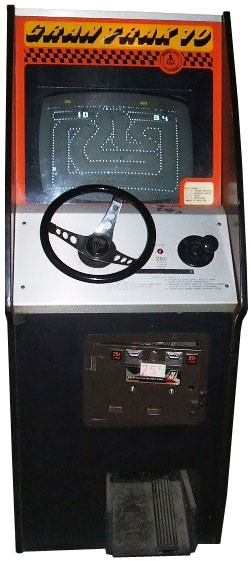
\includegraphics[scale=.33]{Arcade1} 
\caption{A photo of the Atari Gran Trak 10 from 1974, the first arcade vehicle game to utilize steering wheel. }
\label{fig:Arcade}
\end{figure}
\bigskip

None of the major motion capture game systems such as the Wii, Playstation Move, or Xbox Kinect, comes with a steering-wheel contraption specifically usable for vehicle-oriented games such as racing games. However, there are several examples of console enhancements that will allow the player to incorporate the steering wheel into their game style, enhancing the game-experience and unlock the natural feeling of controlling, most often, a motorized vehicle\parencite{Herz1997}.
\bigskip

Where the Wii offers a solution that is compatible with the standard controllers, the Xbox 360 Kinect requires the purchase of an additional controller, which is steering-wheel shaped. Important to note is, that the steering wheel is an independent controller, hence it is does not interact with the Kinect camera. For this particular reason it rather resembles earlier generations of console/PC-steering wheel-controllers, neither which relied on motion tracking by camera.
\bigskip

In between the two is the PlayStation Move Racing Wheel, which is a hybrid of both the Nintendo Wii; and the Kinect steering wheel. Like the Wii, the Move Racing Wheel utilizes the preexisting game-controller, but includes additional functions/relocation of buttons, haptic feedback through vibration, to optimize the game experience.

\subsubsection{Steering wheel functionalities}
\subsubsection*{Introduction}
To account for the functionalities and usage of the controllers, this section covers the remote functionalities of the Wii controller, the Xbox 360 wheel controller and the PlayStation Move wheel controller. This information will make it possible to delimit the functionalities of the games that are developed to that specific console, and therefore controller, since there can only be as much functionality as the controllers support, in terms of buttons and/or motion control as there is available to the specific controller.

\pagebreak[2]

\subsubsection*{Wii Wheel}
\parencite{Nintendo2013}

\begin{figure}[!htbp]
\centering
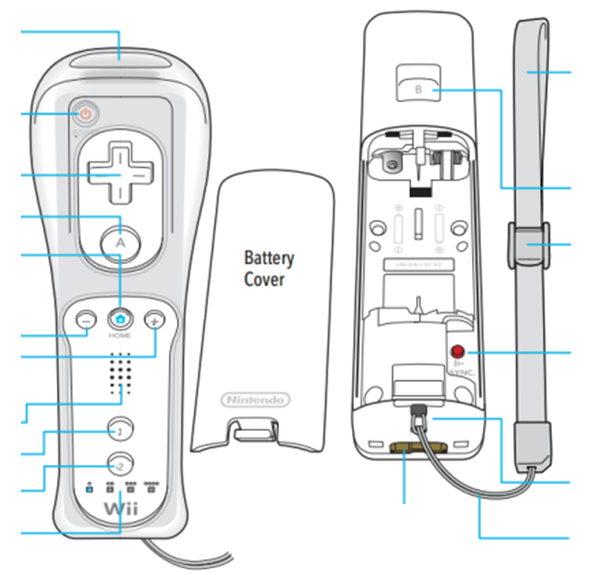
\includegraphics[scale=1]{WiiWheel} 
\caption{Wii Wheel \parencite{Nintendo2013}}
\label{fig:Wiimote}
\end{figure}
\bigskip

As seen in Figure \ref{fig:Wiimote}; The Wii remote functionalities are listed in terms of functionalities and components. The Wii remote is mostly controlled through movement and gestures, so there is only a limited amount of buttons on the controller. These buttons control:
\begin{itemize}
\item Control pad (Up, Down, Left, Right)
\item Pointer lens (the method for registering the controller movement)
\item A. \& B. Button
\item Home Button
\item Minus, Plus button
\item 1. \& 2. Button
\end{itemize}
\bigskip

\pagebreak[2]

\subsubsection*{Xbox 360 wheel controllers}
\parencite{Xbox2013}

\begin{figure}[p]
\centering
\caption{Xbox wheel controller description \parencite{Xbox2013}}
\label{fig:XboxWheel}
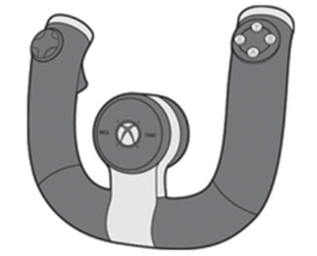
\includegraphics[scale=2]{XboxWheel} 
\end{figure}
\begin{figure}[p]
\centering
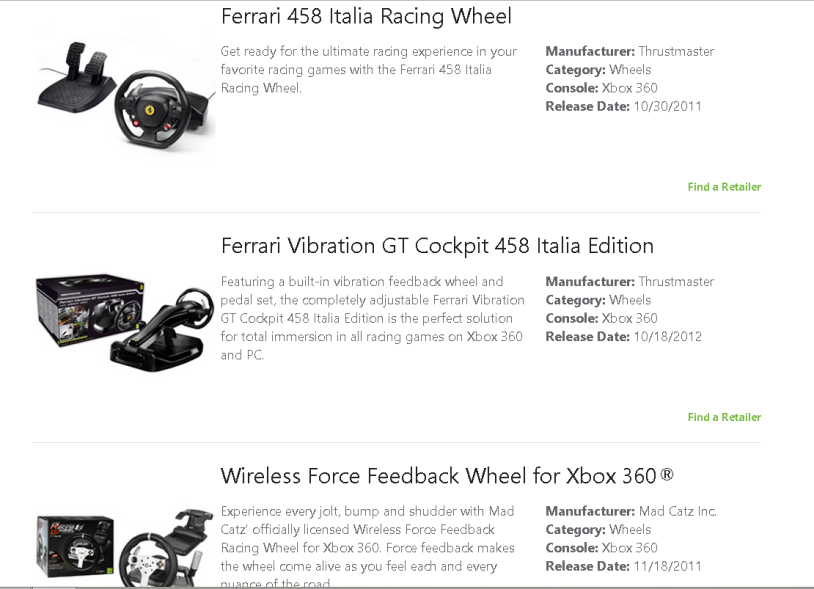
\includegraphics[scale=2]{XboxWheel2}
\caption{Xbox vehicle game controllers. \parencite{Xbox2013}}
\label{fig:XboxWheel2}
\end{figure}

As described in figure \ref{fig:XboxWheel}; The Xbox wireless Speed Wheel contains the following features and functionalities:

\begin{itemize}
\item Vibrating feedback
\item Movement tracking sensors
\item Release buttons for acceleration and braking
\item Buttons for game-defined functionalities (Standard Xbox controller functionalities)
	\begin{itemize}
		\item Standard A, B, X, and Y buttons for game-defined functionalities
		\item Navigation-Button (left, right, up, down)
		\item Guide, start, back (console control buttons)
	\end{itemize}
\end{itemize}

In addition, there are numerous steering wheel controllers compatible with Xbox that utilizes the same as above mentioned functionalities, but also included features such as floor pedals (throttle, brake, clutch) along with gear controller. See figure \ref{fig:XboxWheel2}. for a list of examples.
\bigskip

\pagebreak[4]

\subsubsection*{PlayStation Move wheel controllers}
\parencite{Move2013}

\begin{figure}[!htbp]
\centering
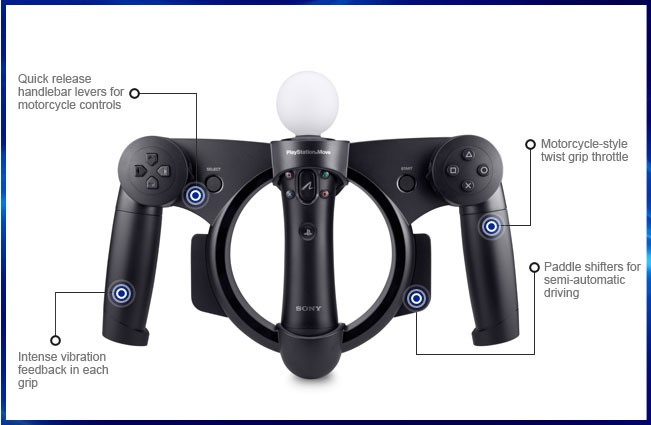
\includegraphics[scale=.1]{MoveWheel}
\caption{PlayStation Move Racing Wheel functionalities \parencite{Move2013}}
\label{fig:MoveWheel}
\end{figure}

As seen in figure \ref{fig:MoveWheel}; The functionalities of the controller are as followed:

\begin{itemize}
\item Vibrating feedback
\item Movement tracking sensors
\item Quick release handlebar levers for motorcycle controls
\item Paddle shifters for semi-automatic driving
\item Buttons for game-defined functionalities (Standard PlayStation controller functionalities)
	\begin{itemize}
	\item Buttons: square, triangle, circle, cross
	\item Navigation-Button (left,right,up,down)
	\item Start \& Select ( console control buttons)
	\end{itemize}
\end{itemize}

\subsubsection*{Summary}
This section describes how the steering wheel controller has been developed to resemble a more realistic and intuitive experience when engaging in vehicle based gameplay. There is also accounted for the design in terms of functionalities of the Wii wheel controller, Xbox 360 wheel controller and PlayStation wheel controllers. This section covers the buttons and other controls of each controller to delimit the plausible amount of functionalities that can be implemented in possible gameplay with each controller.